\documentclass[../Master.tex]{subfiles}
\begin{document}


Our model for our knowledge on conditional effects is similar to
our knowledge of non-conditional actions, for preconditions we operate
with four sets:
\begin{description}
	\item [{Unknown~$B_u$}] The set of all bindings which has
	neither been proven or disproven. As explained in Definition \ref{thm:binding-set}.
	\item [{Proven~$B_k$}] The set of all bindings which has been
	proven.
	\item [{Candidates~C}] Is a set of sets, where each set contains a set $B_c$
	of bindings in which atleast one of the bindings is an actual binding.
	This set like for non-conditional actions are used to prove bindings,
	by disproving the other candidates in the set.
	\item [{Disproven~D}] Is the set of bindings and predicates which have
	been disproven, it can be derived from $D=\left(B_u\cup B_k\right)^{c}$.
\end{description}
These four sets are valuable when discussion what to learn but unfortunately
they are theoretical constructs as modelling compositions of bindings
between predicates has certain difficulties. As shown in Example \ref{thm:sokoban-2}.

	
	\subsection*{Hypergraph}
	
	As we showed earlier what is important when modelling the precondition
	is the expression of the bindings where as the exact names of the
	variables only acts as a hindrance to matching two different sets
	of precondition. Thus a model is needed where the bindings between
	the predicates are what is relevant. For this reason we choose to
	model the recorded unknown preconditions as a hypergraph; in this
	model a node is a single predicate's variable position, and there
	are two kinds of edges, one to bind predicate nodes into a single
	predicate and one to represent the binding between the variables.
	
	The two kinds of edges are as follows: 
	\begin{enumerate}
		\item A single predicate is represented as several nodes one for each variable
		it has. A number is then used to indicate the order of the variable's
		position which is appended to the label of the node. We choose to
		visualize this type of edge with a line.\\
		\begin{tabular}{|c|c|}
			\hline 
			$p(\bot,\bot)$ becomes & 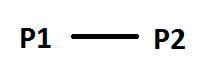
\includegraphics[width=3cm]{../Graphics/connected_nodes}
			\tabularnewline
			\hline 
		\end{tabular}
		\item To represent variables binded together through a common variable we
		choose to visualize this using a bubble around them.\\
		\begin{tabular}{|c|c|}
			\hline 
			p(x) $\land$q(x) becomes & 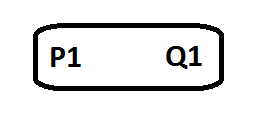
\includegraphics[width=3cm]{../Graphics/connected_binding}\tabularnewline
			\hline 
		\end{tabular}
	\end{enumerate}
	\begin{figure}
		%\includegraphics{house_hypergraph}
		
		\caption{\label{fig:Sokoban-as-hypergraph}Sokoban as hypergraph for Example \ref{thm:sokoban-hypergraph}}
		
	\end{figure}
	
\newtheorem{thm-sokoban-hypergraph}{Example}[section]
\begin{thm-sokoban-hypergraph}\label{thm:sokoban-hypergraph}
	Consider Example \ref{thm:sokoban-example-initial-precond}. In this we had 
	\begin{align*}
		U_p =
		\left\{
			\begin{gathered} 
				\texttt{adj-h}(x, y) \land \texttt{adj-h}(y, z) \land 
				\\ \texttt{box}(y) \land \texttt{at}(z) 
			\end{gathered}
		\right\}
	\end{align*}
	To see this represented as a hypergraph see \figref{House-example-as-hypergraph},
	by modelling this as a graphic the idea of disproving bindings also
	becomes clearer as it literally means to cut an unnecessary edge,
	by removing the node from its binding edge set.
\end{thm-sokoban-hypergraph}
	

\end{document}
